\documentclass[12pt, a4paper]{article}

\usepackage[utf8]{inputenc}
% Limit the page margin to only 1 inch.
\usepackage[margin=1in]{geometry}

%Imports biblatex package
\usepackage[
backend=biber,
style=alphabetic
]{biblatex}
\addbibresource{../../algs4e.bib}

% Enables the `align' environment.
\usepackage{amsmath}
% Provides useful environments, such as:
% - \begin{proof} ...\end{proof}
\usepackage{amsthm}
\usepackage[most]{tcolorbox}

\newtheorem*{proposition}{Proposition}

% Enables using \mathbb{}, for example \mathbb{N} for the set of natural numbers.
\usepackage{amssymb}

% Allows using letters in enumerate list environment. Use, for example:
%\begin{enumerate}[label=(\alph*)]
% ...
%\end{enumerate}
\usepackage[inline]{enumitem}

% Enable importing external graphic files and provides useful commannds, like \graphicspath{}
\usepackage{graphicx}
% Images are located in a directory called images in the current directory.
\graphicspath{{./images/}}

% Make links look better by default.
% See: https://tex.stackexchange.com/questions/823/remove-ugly-borders-around-clickable-cross-references-and-hyperlinks
\usepackage[hidelinks]{hyperref}
\usepackage{xcolor}
\hypersetup{
	colorlinks,
	linkcolor={red!50!black},
	citecolor={blue!50!black},
	urlcolor={blue!80!black}
}


% Code Listings. Source:
% https://stackoverflow.com/questions/3175105/inserting-code-in-this-latex-document-with-indentation
\usepackage{listings}
\usepackage{color}

\definecolor{dkgreen}{rgb}{0,0.6,0}
\definecolor{gray}{rgb}{0.5,0.5,0.5}
\definecolor{mauve}{rgb}{0.58,0,0.82}

\lstset{frame=tb,
	language=Java,
	aboveskip=3mm,
	belowskip=3mm,
	showstringspaces=false,
	columns=flexible,
	basicstyle={\small\ttfamily},
	numbers=none,
	numberstyle=\tiny\color{gray},
	keywordstyle=\color{blue},
	commentstyle=\color{dkgreen},
	stringstyle=\color{mauve},
	breaklines=true,
	breakatwhitespace=true,
	tabsize=3
}

\newcommand{\prob}{\text{P}}
%\newcommand{\complement}{\mathsf{c}}

% Define an environment called "ex" (for Exercise) so that I can do: \begin{ex}{1.5}...\end{ex}
\newenvironment{ex}[2][Exercise]
{\par\medskip\noindent \textbf{#1 #2.}}
{\medskip}

% Define a solution environment, similar to ex (exercise) environment.
\newenvironment{sol}[1][Solution]
{\par\medskip\noindent \textbf{#1.} }
{\medskip}

\begin{document}
	\noindent Sergio E. Garcia Tapia \hfill
	
	\noindent \emph{Algorithms} by Sedgewick and Wayne (4th edition) \cite{sedgewick_wayne}\hfill
	
	\noindent January 16, 2025\hfill 
	\section*{4.3: Minimum Spanning Trees}
	\begin{ex}{1}
		Prove that you can rescale the weights by adding a positive constant to all of them
		or by multiplying them by a positive constant without affecting the MST.
	\end{ex}
	\begin{sol}
		\begin{proof}
			Suppose $G$ is a connected graph. Then $G$ admits an  MST. Let $T$ be
			any MST of $G$.
			
			Let $G_c$ be the graph obtained by adding the positive constant $c$
			to the weight of every edge of $G$. Since the endpoints of the
			edges remain unchanged, it follows that $G_c$ is still connected,
			and thus it admits a spanning tree. In particular, if $T_c$
			is the tree whose edges are the same as $T$ but with weights
			increased by $c$, then $T_c$ is still a spanning tree. To see that it
			is an MST for $G_c$, let $T_c'$ be any other tree spanning tree
			of $G_c$. Let $e_{1,c},\ldots,e_{V-1,c}$ be the edges of $T_c$
			and $f_{1,c},\ldots,f_{V-1,c}$ be the edges of $T_c'$. By definition
			of $G_c$, there are edges $e_k$ and $f_k$ of $G$ satisfying
			\begin{align*}
				w(e_{k,c}')&=w(e_{k}) + c,\\
				w(f_{k,c}')&=w(f_{k}) + c,\\
			\end{align*}
			where $1\leq k\leq V-1$. In particular, the our definition of $T_c$ says that
			$e_1,\ldots,e_{V-1}$ are the edges of $T$, an MST of $G$. Similarly,
			since $T_c'$ is a spanning tree of $G_c$, the edges $f_1,\ldots,f_{V-1}$
			are the same edges but with lower weight. The upshot is that they form
			a spanning tree $T'$ of $G$. By definition of an MST, we know that
			\begin{align*}
				w(T)&\leq w(T')\\
				\sum_{k=1}^{V-1}w(e_k)& \leq \sum_{k=1}^{V-1}w(f_k)\\
				(V-1)\cdot c + \sum_{k=1}^{V-1}w(e_k)& \leq (V-1)\cdot c\sum_{k=1}^{V-1}w(f_k)\\
				\sum_{k=1}^{V-1}(w(e_k) + c)& \leq \sum_{k=1}^{V-1}(w(f_k) + c)\\
				\sum_{k=1}^{V-1}w(e_k')& \leq \sum_{k=1}^{V-1}w(f_k')\\
				w(T_c)&\leq w(T_c')
			\end{align*}
			We conclude that if $T$ is a minimum spanning tree of $G$, the $T_c$ is
			a minimum spanning tree of $G_c$, so the MST is unaffected when all
			edge weights are increased by a positive constant. A similar argument
			works when multiplying by a positive constant.
		\end{proof}
	\end{sol}
	\begin{ex}{2}
		Draw all of the MSTs of the graph depicted in Figure~\ref{fig:ex-02} (all edge weights
		are equal).
		\begin{figure}
			\centering
			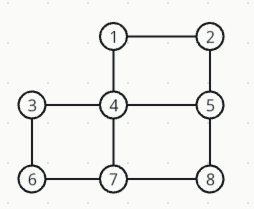
\includegraphics[width=0.2\textwidth]{exercise-02}
			\caption{Undirected edge-weighted graph with all equal weights for Exercise 1.}
			\label{fig:ex-02}
		\end{figure}
	\end{ex}
	\begin{sol}
		Since the graph has $V=8$ vertices, a spanning tree would have $V-1=7$
		edges. The graph is connected with $E=10$ edges, so we need to pick
		$3$ edges to remove. Thus, an upper bound for the number of minimum spanning
		trees is $\binom{10}{3}$. This upper-bound is conservative because we cannot
		just remove \emph{any} edges, given that we also must ensure the graph remains
		connected (else it would not be a spanning tree). Figure~\ref{fig:ex-02-solution} shows
		some, but not all of them.
		\begin{figure}
			\centering
			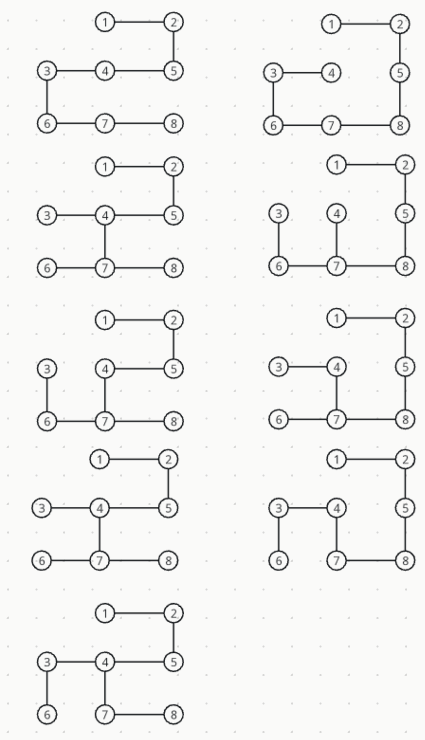
\includegraphics[width=0.4\textwidth]{exercise-02-solution}
			\caption{Some MSTs for the weighted graph in Figure~\ref{fig:ex-02}.}
			\label{fig:ex-02-solution}
		\end{figure}
	\end{sol}
	\begin{ex}{3}
		Show that if a graph's edges all have distinct weights, the MST is unique.
	\end{ex}
	\begin{sol}
		\begin{proof}
			Suppose $T_1$ and $T_2$ are MSTs of a graph $G$ whose edge weights
			are all distinct. Let $e$ be any edge in $T_1$, and suppose that
			$e$ is not in $T_2$. If we add $e$ to $T_2$, then a cycle containing
			$e$ is formed. Let $f$ be any other edge in that cycle, and add
			that edge to $T_1$, thus forming a cycle in $T_1$. By assumption,
			we know that $e$ and $f$ have distinct weights, so without loss
			of generality, suppose $w(e)<w(f)$.
			
			If we remove $f$ from $T_2$, then we eliminate the cycle that was formed
			by adding $e$ to $T_2$, and the tree remains connected. However, now the weight
			of the resulting tree is $w(T_2)-w(e)+w(f)$, which is strictly smaller
			than the weight of $w(T_2)$ because $-w(e)+w(f)<0$. But $T_1$ and
			$T_2$ are MSTs, so this contradicts their minimality.
			
			We conclude that no such each $e$ exists. That is, we do in fact have
			$e\in T_2$. Since $e$ is an arbitrary edge, this hold for every edge of $T_1$.
			A symmetric arguments holds that shows that every edge of $T_2$
			belongs to $T_1$, and hence, $T_1$ and $T_2$ are in fact the
			same tree.
		\end{proof}
	\end{sol}
	\begin{ex}{4}
		Consider the assertion that an edge-weighted graph has a unique MST \emph{only} if
		its edge weights are distinct. Give a proof or a counterexample.
	\end{ex}
	\begin{ex}{5}
		Show that the greedy algorithm is valid even when the edge weights are not distinct.
	\end{ex}
	\begin{ex}{6}
		Give the MST of the weighted graph obtained by deleting vertex \texttt{7} from
		\texttt{tinyEWG.txt} (see page 604).
	\end{ex}
	\begin{ex}{7}
		How would you find a \emph{maximum}s spanning tree of an edge-weighted graph?
	\end{ex}
	\begin{ex}{8}
		Prove the following, known as the \emph{cycle property}: Given any cycle in an
		edge-weighted graph (all edge weights distinct), the edge of maximum weight in
		the cycle does not belong to the MST of the graph.
	\end{ex}
	\begin{ex}{9}
		Implement the constructor for \texttt{EdgeWeightedGraph} that reads an edge-weighted
		graph from the input stream, by suitably modifying the constructor from \texttt{Graph}
		(see page 526).
	\end{ex}
	\begin{ex}{10}
		Develop an \texttt{EdgeWeightedGraph} implementation for dense graphs that uses an
		adjacency matrix (two-dimensional array of weights) representation. Disallow parallel
		edges.
	\end{ex}
	\begin{ex}{11}
		Determine the amount of memory used by \texttt{EdgeWeightedGraph} to represent a graph
		with $V$ vertices and $E$ edges, using the memory-cost model of \textbf{Section 1.4}.
	\end{ex}
	\begin{ex}{12}
		Suppose that a graph has distinct edge weights. Does its lightest edge have to belong
		to the MST? Can its heaviest edge belong to the MST? Does a min-weight edge on
		every cycle have to belong to the MST? Prove your answer to each question or give
		a counterexample.
	\end{ex}
	\begin{ex}{13}
		Give a counterexample that shows why the following strategy does not necessarily
		find the MST: ``Start with any vertex as a single-vertex MST, the add \texttt{V-1}
		edges to it, always taking next a min-weight edge incident to the vertex most
		recently added to the MST."
	\end{ex}
	
	\pagebreak
	\printbibliography
\end{document}